\documentclass[12pt,a4paper]{article}
\usepackage{fullpage}
\usepackage[margin=2cm]{geometry}
\usepackage{amsmath}
\usepackage{subfig}
\usepackage{graphicx}
\usepackage[justification=centering]{caption}
\usepackage{multicol}

\begin{document}
\title{Fine-tuning CNN on Beetles dataset }
\author{LE Van Linh and BEURTON-AIMAR Marie}
\date{March, 2018}
\maketitle
\begin{abstract}
In this study, we continue applying the convolutional neural network (CNN) to predict the landmarks on other parts of beetles, i.e, pronotum, head and body. The proposed model was continuing to use to predict the landmarks. However, instead of training from scratch on each dataset, the model has been training with a combined data of three parts: pronotum, head and body part (called training stage); then, the trained model is used to fine-tune on each dataset and predict the landmarks (called fine-tuning stage). In training stage, $260$ images have been chosen randomly on each part. Then, they are enlarged to obtain $5460$ images ($260 \times 7 \times 3$) which are used to train the network. In fine-tuning stage, the trained model has been fine-tuned on each dataset. After fine-tuning, the model is used to predict the landmarks of the images in the test set. The coordinates of predicted landmarks are evaluated by calculating the distance between manual landmarks and corresponding predicted landmarks. The model is implemented by Python on Lassagne framework\cite{lasagne}.
\end{abstract}

\section{Model architecture and training stage}
\subsection{Architecture}
The network includes three convolutional(CONV) layers followed by three maximum pooling(POOL) layers, four dropouts(DROP) layers, and three full connected(FC) layers (Fig.\ref{pmodel}). The input of the network is the gray-scale image with the size of $256 \times 192$. The depth of network can be expressed by increasing of the deep at each convolutional layer. They are increased from $32, 64,$ and $128$ from the first CONV layer to the third CONV layer with different filter sizes. While, the filter sizes are kept in the same size for every POOL layers. The dropout ratios of the DROP layers increase from the first to the end: $0.1, 0.2, 0.3, $ and $0.5$. At the end of the network, three full connected are set up to predict the landmarks. The first two FC layers have the same outputs($1000$) while the output at the last FC has been change to correspond with the number of landmarks. The detail parameters at each layer are presented in Appendix \ref{apa}. The model is implemented by Lassagne framework\cite{lasagne}.
\begin{figure}[h!]
	\centering
	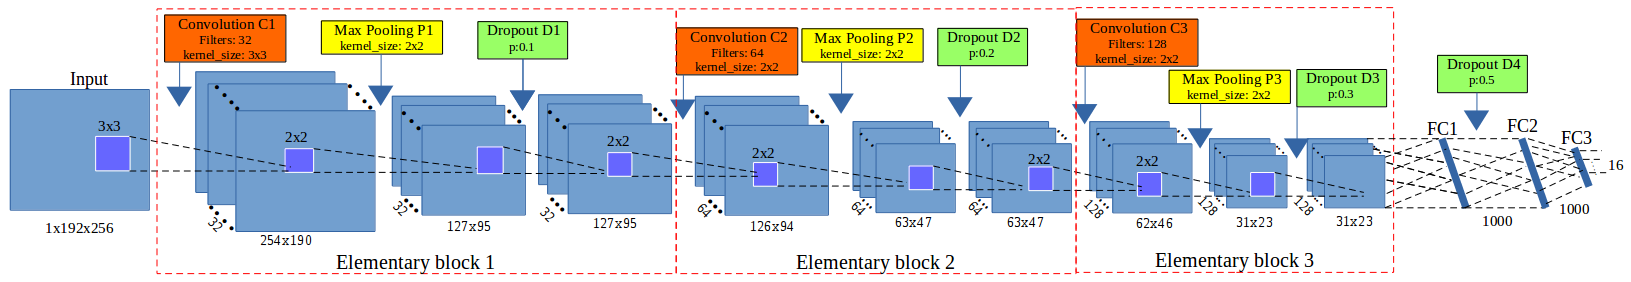
\includegraphics[scale=0.3]{images/fine_tuning/arch_model}
	\caption{The illustration of the convolutional neural network}
	\label{pmodel}
\end{figure}
\subsection{Parameters}
The model is trained with $10000$ \texttt{epochs} and \texttt{batch size} of $128$ (default value of Lasagne). For each epoch, the dataset is randomly split into training set and validation set with the ratio of $0.6:0.4$. The \texttt{learning rate} and \texttt{momentum} are initialized to $0.01$ and $0.9$, respectively. During training, they are re-calculated to adjust with the remaining epochs. All the initial parameters are shown in the Table \ref{initparameters}.
\begin{table}[h!]
	\centering
	\begin{tabular}{l l l}
	Parameter & Initial value & End value \\ \hline
	Epochs & $10000$ &  \\ \hline
	Training batch size & $128$ & \\ \hline
	Testing batch size & $128$ & \\ \hline
	Learning rate & $0.01$ & $0.0001$ \\ \hline
	Momentum & $0.9$ & $0.9999$ \\ \hline
	\end{tabular}
	\caption{The network parameters in proposed model}
	\label{initparameters}
\end{table}
\subsection{Training data}
The training data is combined from the images of three parts: \textit{pronotum, body, head}. For each part, $260$ original images have been chosen randomly ($260 \times 3 = 780$). Then, the number of images have been enlarged by applying two procedures. 

The \textbf{first} procedure is adding a constant value to a channel of RGB image, we will have a new RGB image. For example, from an original $RGB$ image, if we add $10$ to red channel, we will have a new image $(R+10)GB$. Then, we apply the same rule with blue and green channel, we will obtain two new images: $R(G+10)B$ and $RG(B+10)$. By that way, from an RGB image, we can generate three RGB images by adding a constant to each channel(each time just change to a channel). 

The \textbf{second} procedure is splitting the channels of RGB image (because the models work on gray-scale). It means that we can generate six versions from an original image. At the end, the number of the image in the training data is $ 260 \times 3 \times 7 = 5460$ images (six versions and original). Before giving to the models, the images are down-sampled with the size of $256 \times 192$. The number of the images in training set and validation set are splitted automatically by the model's parameter.

After generating the images, the dataset is large enough to train with CNN. However, another problem has occurred that the number of landmarks of each part is different: \textit{8 landmarks on pronotum part, 11 landmarks on body part, and 10 landmarks on head}. Because the location of the landmarks has a signification with biologists, so, adding the landmarks are more difficult than removing the landmarks. Therefore, we kept the number of landmarks on pronotum as a reference and we suppressed the landmarks on body and head part. Specifically, we have removed $3$ landmarks on body part ($1^{st}, 6^{th}, 9^{th}$) and $2$ landmarks on head part($5^{th}, 6^{th}$).

\subsection{Training process}
The model has been trained on the dataset including the images of 3 parts. The training process was finished in $10000$ epochs. Figure.\ref{ptlosses} shows the losses during training process (training loss and validation loss). At the beginning, the validation loss is always higher than the tranining loss, but from the 2000 epochs, the training loss begins stable while the validation loss continue to decrease. At the end of training, the losses values are $0.00029$ and $0.00009$ for training and validation, respectively.
\begin{figure}[h!]
	\centering
	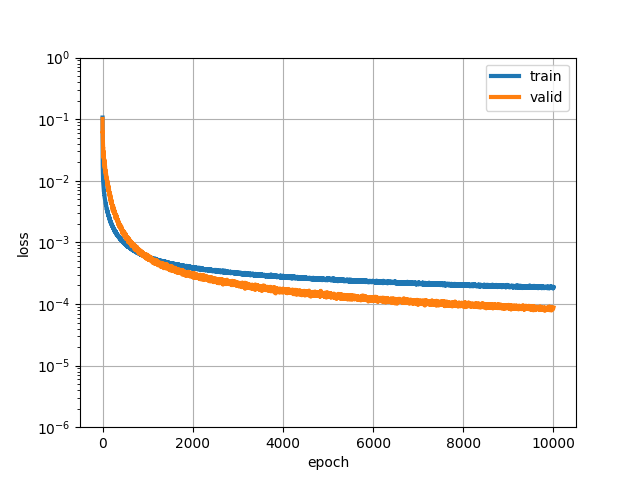
\includegraphics[scale=0.7]{images/fine_tuning/all_parts_10000epochs}
	\caption{The losses during training process}
	\label{ptlosses}
\end{figure}

\section{Fine-tuning stage}
The trained model have been continued to fine-tune\cite{} on each dataset: pronotum, body, and head. For each part, to get all predicted landmarks for all images, a scenario (called round) has been applied to choose $33$ images for the test set, the remaining images have been put to the training set. After fine-tuning, the model has abled to predict the landmarks corresponds to each part of beetles.

In the next, each sub-section includes two tables: the first table presents the losses during fine-tuning on each dataset; the second table presents the comparison based on the average distances (in pixels) of two different procedures (fine-tuning and training from scratch). The average distances are given by each landmarks.

\subsection{Pronotum dataset}
Table.\ref{tblftpronotum} shows the losses during fine-tuning the trained model on pronotum dataset.
\begin{table}[htbp]
\begin{minipage}[b]{.5\textwidth}
	\centering
	\begin{tabular}{l l l}
	Round & Training loss & Validation loss \\ \hline
	1 & 0.00019 & 0.00009  \\ \hline
	2 & 0.00018 & 0.00010 \\ \hline
	3 & 0.00018 & 0.00010 \\ \hline
	4 & 0.00019 & 0.00008 \\ \hline
	5 & 0.00019 & 0.00009 \\ \hline
	6 & 0.00018 & 0.00008 \\ \hline
	7 & 0.00019 & 0.00008 \\ \hline
	8 & 0.00018 & 0.00006 \\ \hline
	9 & 0.00018 & 0.00009 \\ \hline
	\end{tabular}
	\caption{The losses during fine-tuning model on pronotum dataset}
	\label{tblftpronotum}
\end{minipage}
\hfill
\begin{minipage}[b]{.5\textwidth}
\centering
\begin{tabular}{|c|c|c|}
\hline
\textbf{$\#$Landmark} & \textbf{From scratch} & \textbf{Fine-tune} \\ \hline
1 & 4.00 & 2.49  \\ \hline
2 & 4.48 & 2.72  \\ \hline
3 & 4.30  & 2.65 \\ \hline
4 & 4.39  & 2.77 \\ \hline
5 & 4.29  & 2.49 \\ \hline
6 & 5.36  & 3.05 \\ \hline
7 & 4.64  & 2.68 \\ \hline
8 & 4.94  & 2.87 \\ \hline
\end{tabular}
\caption{The average error distance per landmark.}
\label{tblcmppronotum}
\end{minipage}
\end{table}

To have a comparison with the last result (training from scratch), the fine-tuned model has been used to predict the landmarks on protum images. Then, the distance between the manual landmarks and corresponding predicted landmarks has been computed. Table.\ref{tblcmppronotum} shows the average distances which given by each landmark. The values is \textbf{Fine-tune} columns presents for the average distance of fine-tuned model, while \textbf{From scratch} columns presents for the average distance of the last result (train model from scratch on pronotum dataset).

\subsection{Body dataset}
Table.\ref{tblftbody} shows the losses during fine-tuning the trained model on body dataset. Table.\ref{tblcmpbody} shows the comparison on average distance between two periods.
\begin{table}[ht]
\begin{minipage}[b]{0.5\textwidth}
	\centering
	\begin{tabular}{c c c}
	Round & Training loss & Validation loss \\ \hline
	1 & 0.00020 & 0.00006  \\ \hline
	2 & 0.00020 & 0.00006 \\ \hline
	3 & 0.00021 & 0.00006 \\ \hline
	4 & 0.00021 & 0.00006 \\ \hline
	5 & 0.00019 & 0.00006 \\ \hline
	6 & 0.00019 & 0.00006 \\ \hline
	7 & 0.00018 & 0.00005 \\ \hline
	8 & 0.00020 & 0.00006 \\ \hline
	9 & 0.00019 & 0.00006 \\ \hline
	\end{tabular}
	\caption{The losses during fine-tuning model on body dataset}
	\label{tblftbody}
\end{minipage}
\hfill
\begin{minipage}[b]{0.5\textwidth}

\centering
\begin{tabular}[t]{|c|c|c|}
\hline
\textbf{$\#$Landmark} & \textbf{From scratch} & \textbf{Fine-tune} \\ \hline
1 & 3.87 & 2.34  \\ \hline
2 & 3.97 & 2.27  \\ \hline
3 & 3.92  & 2.27 \\ \hline
4 & 3.87  & 2.25 \\ \hline
5 & 4.02  & 2.27 \\ \hline
6 & 4.84  & 3.14 \\ \hline
7 & 5.21  & 3.14 \\ \hline
8 & 5.47  & 3.29 \\ \hline
9 & 5.27  & 3.42 \\ \hline
10 & 4.07  & 2.49 \\ \hline
11 & 3.99  & 2.30 \\ \hline
\end{tabular}
\caption{The average error distance per landmark.}
\label{tblcmpbody}

\end{minipage}
\end{table}
\subsection{Head dataset}
Table.\ref{tblfthead} shows the losses during fine-tuning the trained model on head dataset. Table.\ref{tblcmphead} shows the comparison on average distance between two periods.

\begin{table}[ht]
\begin{minipage}[b]{0.5\textwidth}
	\centering
	\begin{tabular}{l l l}
	Round & Training loss & Validation loss \\ \hline
	1 & 0.00022 & 0.00007  \\ \hline
	2 & 0.00022 & 0.00007 \\ \hline
	3 & 0.00023 & 0.00008 \\ \hline
	4 & 0.00023 & 0.00008 \\ \hline
	5 & 0.00022 & 0.00008 \\ \hline
	6 & 0.00023 & 0.00007 \\ \hline
	7 & 0.00022 & 0.00008 \\ \hline
	8 & 0.00023 & 0.00007 \\ \hline
	9 & 0.00024 & 0.00008 \\ \hline
	\end{tabular}
	\caption{The losses during fine-tuning model on head dataset}
	\label{tblfthead}
\end{minipage}
\hfill
\begin{minipage}[b]{0.5\textwidth}
\centering
\begin{tabular}{|c|c|c|}
\hline
\textbf{$\#$Landmark} & \textbf{From scratch} & \textbf{Fine-tune} \\ \hline
1 & 5.53 & 3.03  \\ \hline
2 & 5.16 & 2.94  \\ \hline
3 & 5.38  & 2.96 \\ \hline
4 & 5.03  & 2.88 \\ \hline
5 & 4.84  & 2.76 \\ \hline
6 & 4.45  & 2.67 \\ \hline
7 & 4.79  & 2.29 \\ \hline
8 & 4.53  & 2.20 \\ \hline
9 & 5.14  & 2.57 \\ \hline
10 & 5.06  & 2.44 \\ \hline
\end{tabular}
\caption{The average error distance per landmark.}
\label{tblcmphead}
\end{minipage}
\end{table}

\section{Conclusions}
In this study, we proposed a CNN to predict the landmarks on beetles images. The model is trained on a combining data of $3$ parts: pronotum, head, and body. Then, the trained model has been used to fine-tune on each dataset. The fine-tuned models are used to predict the landmarks on the correspoding testing dataset. The coordinates of predicted landmarks are evaluated by calculating the distance to the manual ones. The study presents also a comparison between two different procedures for each dataset (training from scratch and fine-tuning). The experiments result can be download from GitHub\footnote{https://github.com/linhlevandlu/cnnBeetles}. The explaination about structure are given in appendix part.
\bibliographystyle{unsrt}
\bibliography{includes/references}
\pagebreak
\appendix
\begin{center}
\textbf{\LARGE{APPENDIX}}
\end{center}
\section*{Experiment results}
\label{apb}
\begin{itemize}
	\item \textbf{data} folder: contains the results when we train the model from scratch (the last result). All of the experiment results is provided on GitHub. Each folder contains the results corresponding to each beetle's part. In each folder, we provide the losses curves, result images(first sixteen images of each test set), and the prediction landmarks(in csv file). Each folder contains:
\begin{itemize}
	%\item Folder \textbf{models} contains the output models following each training round,
	\item \textbf{Test} folder: contains the loss curves during training (and validation) and the prediction on test images (top 16) for each training round,
	\item \textbf{CSV} file: contains the information of image, index of landmark, coordinates of manual landmark$(x1,y1)$, and coordinates of predicted landmark$(x2,y2)$.
	\item The output trained model can be obtained by requesting the authors.
\end{itemize}
	\item \textbf{fine\_tuning} folder: contains the result when we \textbf{fine-tune the trained model} on each separate dataset. It includes:
		\begin{itemize}
			\item \textbf{csv} folder: contains the distances between the predicted and manual landmarks of all images, which given by each landmark.
			\item \textbf{data} folder: contains some predicted examples (\textit{images}) and the coordinates of all predicted landmarks (\textit{predicted\_landmarks} folder)
			\item \textbf{ods} folder: contains all \textbf{ods} files which provide the statistic processes.
		\end{itemize}
	\item \textbf{latex} folder: contains the latex source of summary documents.
\end{itemize}

\end{document}